\documentclass[../main]{subfiles}
\begin{document}
\setcounter{secnumdepth}{4}
    \chapter{要素技術}
        \section{トポロジカルマップ}
        私たちの身の回りには様々な種類の地図があり,活用されている.
        例えば,に表すメトリックマップと呼ばれる地図は,普段人が目的地まで移動する際に用いられる.
        しかし,本研究で用いているトポロジカルマップはのような形をしている.メトリックマップがやや複雑な形をしているのに対し,
        トポロジカルマップはより簡潔に,環境を抽象的に表現することができる.

        
        トポロジカルマップは,大きく分けてノードとエッジの2つの要素により構成されている.
        Fig~では,赤い丸の図形で表現されているのがノードである.ノードには,地図の作成者が好きな情報を入れることができる.
        もう1つの要素であるエッジは,それぞれのノード同士を接続するのに用いられる.
        ノード同士に関係性がある場合,ノードとノードはエッジにより接続される.
    
        \newpage

        \section{Neural Network}
        \section{Convolutional Neural Network(CNN)}

        \newpage
        
        \section{You Only Look Once(YOLO)}
        本研究で用いるYOLO\cite{yolo_paper_fig}は,リアルタイム物体検出アルゴリズムである.
        YOLOは,画像のRGBデータの配列をCNNに入力し,画像中のどの範囲に物体が存在しているのかを表すバウンディングボックスの情報と,
        ボックス内の物体がどのクラスに属しているのかを確率とともに表すクラス確率の情報を出力する.
        \fref{figure::yolo_exp}は,YOLOを用いて画像中の物体を検出している様子である. 

        \begin{figure}[H]
        \centering
        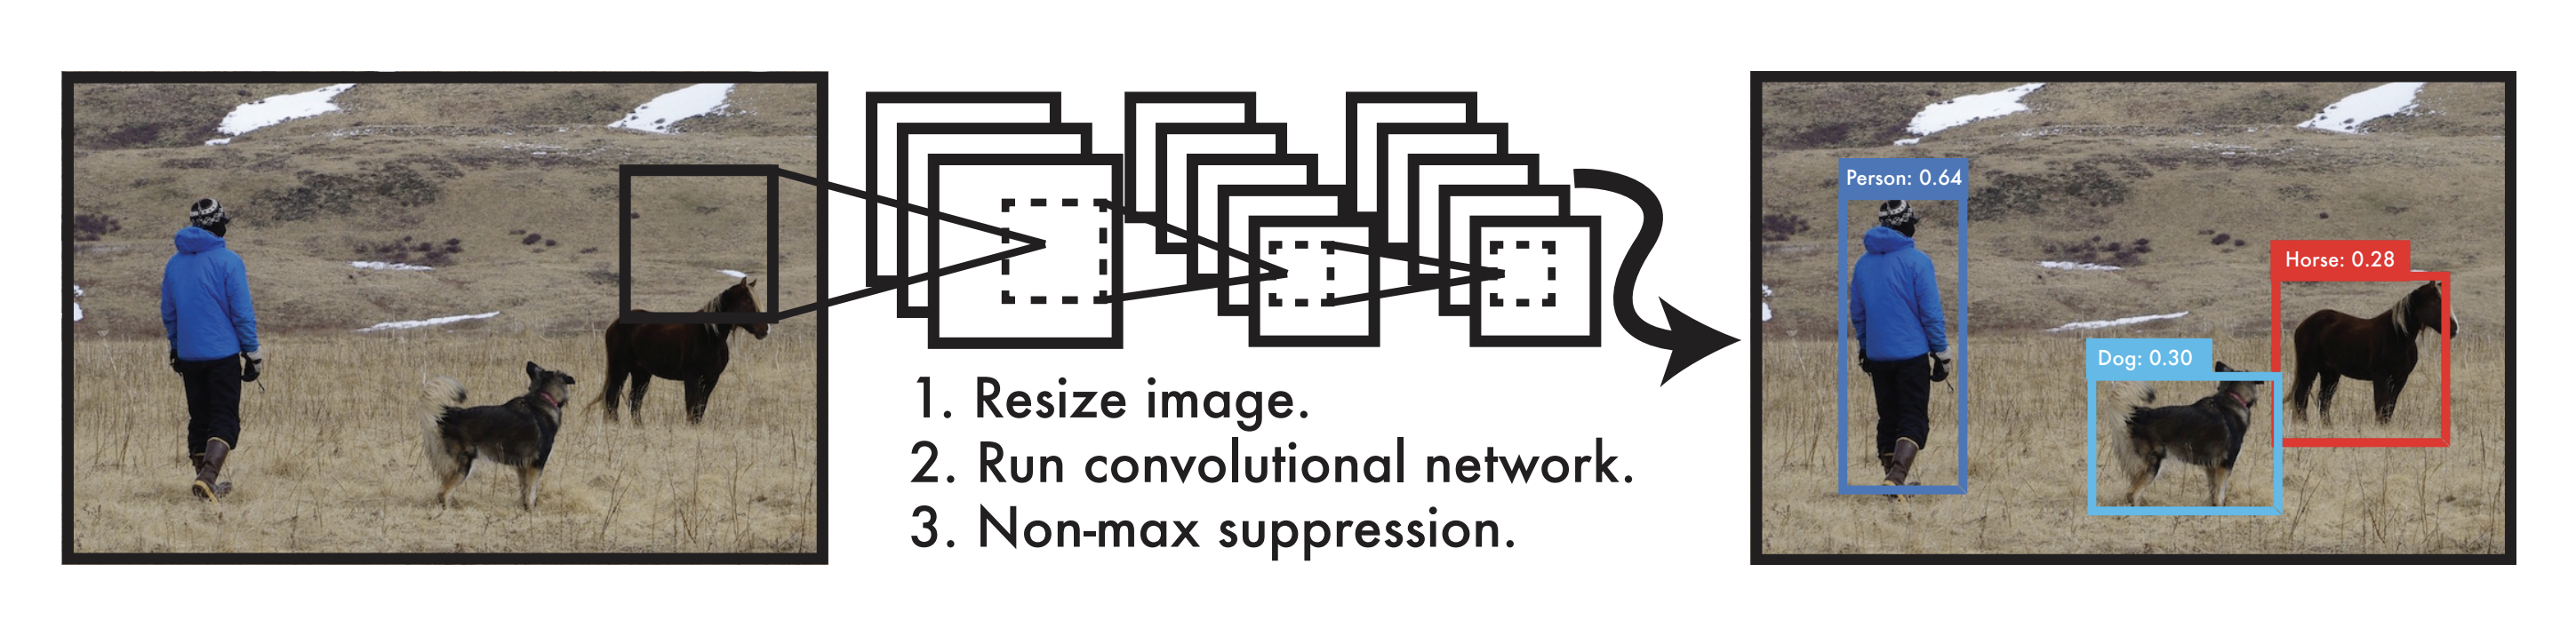
\includegraphics[width=10cm]{../images/yolo_exp.png}
        \caption{The YOLO Detection System.(出典:)}
        \label{figure::yolo_exp}
        \end{figure}
        左の画像データを入力した結果,画像からは3つの物体が検出されている.
        また,それぞれの物体がPerson 0.64,Dog 0.30,Hose 0.28の確率で予測されていることが確認できる.
    \end{document}